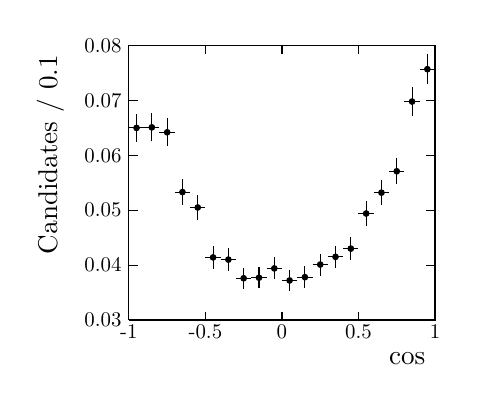
\begin{tikzpicture}
\pgfdeclareplotmark{cross} {
\pgfpathmoveto{\pgfpoint{-0.3\pgfplotmarksize}{\pgfplotmarksize}}
\pgfpathlineto{\pgfpoint{+0.3\pgfplotmarksize}{\pgfplotmarksize}}
\pgfpathlineto{\pgfpoint{+0.3\pgfplotmarksize}{0.3\pgfplotmarksize}}
\pgfpathlineto{\pgfpoint{+1\pgfplotmarksize}{0.3\pgfplotmarksize}}
\pgfpathlineto{\pgfpoint{+1\pgfplotmarksize}{-0.3\pgfplotmarksize}}
\pgfpathlineto{\pgfpoint{+0.3\pgfplotmarksize}{-0.3\pgfplotmarksize}}
\pgfpathlineto{\pgfpoint{+0.3\pgfplotmarksize}{-1.\pgfplotmarksize}}
\pgfpathlineto{\pgfpoint{-0.3\pgfplotmarksize}{-1.\pgfplotmarksize}}
\pgfpathlineto{\pgfpoint{-0.3\pgfplotmarksize}{-0.3\pgfplotmarksize}}
\pgfpathlineto{\pgfpoint{-1.\pgfplotmarksize}{-0.3\pgfplotmarksize}}
\pgfpathlineto{\pgfpoint{-1.\pgfplotmarksize}{0.3\pgfplotmarksize}}
\pgfpathlineto{\pgfpoint{-0.3\pgfplotmarksize}{0.3\pgfplotmarksize}}
\pgfpathclose
\pgfusepathqstroke
}
\pgfdeclareplotmark{cross*} {
\pgfpathmoveto{\pgfpoint{-0.3\pgfplotmarksize}{\pgfplotmarksize}}
\pgfpathlineto{\pgfpoint{+0.3\pgfplotmarksize}{\pgfplotmarksize}}
\pgfpathlineto{\pgfpoint{+0.3\pgfplotmarksize}{0.3\pgfplotmarksize}}
\pgfpathlineto{\pgfpoint{+1\pgfplotmarksize}{0.3\pgfplotmarksize}}
\pgfpathlineto{\pgfpoint{+1\pgfplotmarksize}{-0.3\pgfplotmarksize}}
\pgfpathlineto{\pgfpoint{+0.3\pgfplotmarksize}{-0.3\pgfplotmarksize}}
\pgfpathlineto{\pgfpoint{+0.3\pgfplotmarksize}{-1.\pgfplotmarksize}}
\pgfpathlineto{\pgfpoint{-0.3\pgfplotmarksize}{-1.\pgfplotmarksize}}
\pgfpathlineto{\pgfpoint{-0.3\pgfplotmarksize}{-0.3\pgfplotmarksize}}
\pgfpathlineto{\pgfpoint{-1.\pgfplotmarksize}{-0.3\pgfplotmarksize}}
\pgfpathlineto{\pgfpoint{-1.\pgfplotmarksize}{0.3\pgfplotmarksize}}
\pgfpathlineto{\pgfpoint{-0.3\pgfplotmarksize}{0.3\pgfplotmarksize}}
\pgfpathclose
\pgfusepathqfillstroke
}
\pgfdeclareplotmark{newstar} {
\pgfpathmoveto{\pgfqpoint{0pt}{\pgfplotmarksize}}
\pgfpathlineto{\pgfqpointpolar{44}{0.5\pgfplotmarksize}}
\pgfpathlineto{\pgfqpointpolar{18}{\pgfplotmarksize}}
\pgfpathlineto{\pgfqpointpolar{-20}{0.5\pgfplotmarksize}}
\pgfpathlineto{\pgfqpointpolar{-54}{\pgfplotmarksize}}
\pgfpathlineto{\pgfqpointpolar{-90}{0.5\pgfplotmarksize}}
\pgfpathlineto{\pgfqpointpolar{234}{\pgfplotmarksize}}
\pgfpathlineto{\pgfqpointpolar{198}{0.5\pgfplotmarksize}}
\pgfpathlineto{\pgfqpointpolar{162}{\pgfplotmarksize}}
\pgfpathlineto{\pgfqpointpolar{134}{0.5\pgfplotmarksize}}
\pgfpathclose
\pgfusepathqstroke
}
\pgfdeclareplotmark{newstar*} {
\pgfpathmoveto{\pgfqpoint{0pt}{\pgfplotmarksize}}
\pgfpathlineto{\pgfqpointpolar{44}{0.5\pgfplotmarksize}}
\pgfpathlineto{\pgfqpointpolar{18}{\pgfplotmarksize}}
\pgfpathlineto{\pgfqpointpolar{-20}{0.5\pgfplotmarksize}}
\pgfpathlineto{\pgfqpointpolar{-54}{\pgfplotmarksize}}
\pgfpathlineto{\pgfqpointpolar{-90}{0.5\pgfplotmarksize}}
\pgfpathlineto{\pgfqpointpolar{234}{\pgfplotmarksize}}
\pgfpathlineto{\pgfqpointpolar{198}{0.5\pgfplotmarksize}}
\pgfpathlineto{\pgfqpointpolar{162}{\pgfplotmarksize}}
\pgfpathlineto{\pgfqpointpolar{134}{0.5\pgfplotmarksize}}
\pgfpathclose
\pgfusepathqfillstroke
}
\definecolor{c}{rgb}{1,1,1};
\draw [color=c, fill=c] (0.1,0.0918919) rectangle (4.9,4.5027);
\draw [color=c, fill=c] (0.772,0.797622) rectangle (4.66,4.28216);
\definecolor{c}{rgb}{0,0,0};
\draw [c] (0.772,0.797622) -- (0.772,4.28216) -- (4.66,4.28216) -- (4.66,0.797622) -- (0.772,0.797622);
\draw [c,line width=0.4] (0.8692,3.05912) -- (0.8692,3.2368);
\draw [c,line width=0.4] (0.8692,3.2368) -- (0.8692,3.41448);
\draw [c,line width=0.4] (0.772,3.2368) -- (0.8692,3.2368);
\draw [c,line width=0.4] (0.8692,3.2368) -- (0.9664,3.2368);
\foreach \P in {(0.8692,3.2368)}{\draw[mark options={color=c,fill=c},mark size=1.201201pt,mark=*,mark size=1pt] plot coordinates {\P};}
\draw [c,line width=0.4] (1.0636,3.06595) -- (1.0636,3.24377);
\draw [c,line width=0.4] (1.0636,3.24377) -- (1.0636,3.42158);
\draw [c,line width=0.4] (0.9664,3.24377) -- (1.0636,3.24377);
\draw [c,line width=0.4] (1.0636,3.24377) -- (1.1608,3.24377);
\foreach \P in {(1.0636,3.24377)}{\draw[mark options={color=c,fill=c},mark size=1.201201pt,mark=*,mark size=1pt] plot coordinates {\P};}
\draw [c,line width=0.4] (1.258,3.00447) -- (1.258,3.18105);
\draw [c,line width=0.4] (1.258,3.18105) -- (1.258,3.35763);
\draw [c,line width=0.4] (1.1608,3.18105) -- (1.258,3.18105);
\draw [c,line width=0.4] (1.258,3.18105) -- (1.3552,3.18105);
\foreach \P in {(1.258,3.18105)}{\draw[mark options={color=c,fill=c},mark size=1.201201pt,mark=*,mark size=1pt] plot coordinates {\P};}
\draw [c,line width=0.4] (1.4524,2.26052) -- (1.4524,2.42142);
\draw [c,line width=0.4] (1.4524,2.42142) -- (1.4524,2.58231);
\draw [c,line width=0.4] (1.3552,2.42142) -- (1.4524,2.42142);
\draw [c,line width=0.4] (1.4524,2.42142) -- (1.5496,2.42142);
\foreach \P in {(1.4524,2.42142)}{\draw[mark options={color=c,fill=c},mark size=1.201201pt,mark=*,mark size=1pt] plot coordinates {\P};}
\draw [c,line width=0.4] (1.6468,2.06967) -- (1.6468,2.22628);
\draw [c,line width=0.4] (1.6468,2.22628) -- (1.6468,2.38289);
\draw [c,line width=0.4] (1.5496,2.22628) -- (1.6468,2.22628);
\draw [c,line width=0.4] (1.6468,2.22628) -- (1.744,2.22628);
\foreach \P in {(1.6468,2.22628)}{\draw[mark options={color=c,fill=c},mark size=1.201201pt,mark=*,mark size=1pt] plot coordinates {\P};}
\draw [c,line width=0.4] (1.8412,1.4503) -- (1.8412,1.5921);
\draw [c,line width=0.4] (1.8412,1.5921) -- (1.8412,1.7339);
\draw [c,line width=0.4] (1.744,1.5921) -- (1.8412,1.5921);
\draw [c,line width=0.4] (1.8412,1.5921) -- (1.9384,1.5921);
\foreach \P in {(1.8412,1.5921)}{\draw[mark options={color=c,fill=c},mark size=1.201201pt,mark=*,mark size=1pt] plot coordinates {\P};}
\draw [c,line width=0.4] (2.0356,1.42311) -- (2.0356,1.56422);
\draw [c,line width=0.4] (2.0356,1.56422) -- (2.0356,1.70533);
\draw [c,line width=0.4] (1.9384,1.56422) -- (2.0356,1.56422);
\draw [c,line width=0.4] (2.0356,1.56422) -- (2.1328,1.56422);
\foreach \P in {(2.0356,1.56422)}{\draw[mark options={color=c,fill=c},mark size=1.201201pt,mark=*,mark size=1pt] plot coordinates {\P};}
\draw [c,line width=0.4] (2.23,1.19214) -- (2.23,1.32727);
\draw [c,line width=0.4] (2.23,1.32727) -- (2.23,1.46241);
\draw [c,line width=0.4] (2.1328,1.32727) -- (2.23,1.32727);
\draw [c,line width=0.4] (2.23,1.32727) -- (2.3272,1.32727);
\foreach \P in {(2.23,1.32727)}{\draw[mark options={color=c,fill=c},mark size=1.201201pt,mark=*,mark size=1pt] plot coordinates {\P};}
\draw [c,line width=0.4] (2.4244,1.19893) -- (2.4244,1.33424);
\draw [c,line width=0.4] (2.4244,1.33424) -- (2.4244,1.46956);
\draw [c,line width=0.4] (2.3272,1.33424) -- (2.4244,1.33424);
\draw [c,line width=0.4] (2.4244,1.33424) -- (2.5216,1.33424);
\foreach \P in {(2.4244,1.33424)}{\draw[mark options={color=c,fill=c},mark size=1.201201pt,mark=*,mark size=1pt] plot coordinates {\P};}
\draw [c,line width=0.4] (2.6188,1.31438) -- (2.6188,1.45272);
\draw [c,line width=0.4] (2.6188,1.45272) -- (2.6188,1.59105);
\draw [c,line width=0.4] (2.5216,1.45272) -- (2.6188,1.45272);
\draw [c,line width=0.4] (2.6188,1.45272) -- (2.716,1.45272);
\foreach \P in {(2.6188,1.45272)}{\draw[mark options={color=c,fill=c},mark size=1.201201pt,mark=*,mark size=1pt] plot coordinates {\P};}
\draw [c,line width=0.4] (2.8132,1.16498) -- (2.8132,1.2994);
\draw [c,line width=0.4] (2.8132,1.2994) -- (2.8132,1.43381);
\draw [c,line width=0.4] (2.716,1.2994) -- (2.8132,1.2994);
\draw [c,line width=0.4] (2.8132,1.2994) -- (2.9104,1.2994);
\foreach \P in {(2.8132,1.2994)}{\draw[mark options={color=c,fill=c},mark size=1.201201pt,mark=*,mark size=1pt] plot coordinates {\P};}
\draw [c,line width=0.4] (3.0076,1.20572) -- (3.0076,1.34121);
\draw [c,line width=0.4] (3.0076,1.34121) -- (3.0076,1.4767);
\draw [c,line width=0.4] (2.9104,1.34121) -- (3.0076,1.34121);
\draw [c,line width=0.4] (3.0076,1.34121) -- (3.1048,1.34121);
\foreach \P in {(3.0076,1.34121)}{\draw[mark options={color=c,fill=c},mark size=1.201201pt,mark=*,mark size=1pt] plot coordinates {\P};}
\draw [c,line width=0.4] (3.202,1.36194) -- (3.202,1.5015);
\draw [c,line width=0.4] (3.202,1.5015) -- (3.202,1.64105);
\draw [c,line width=0.4] (3.1048,1.5015) -- (3.202,1.5015);
\draw [c,line width=0.4] (3.202,1.5015) -- (3.2992,1.5015);
\foreach \P in {(3.202,1.5015)}{\draw[mark options={color=c,fill=c},mark size=1.201201pt,mark=*,mark size=1pt] plot coordinates {\P};}
\draw [c,line width=0.4] (3.3964,1.45709) -- (3.3964,1.59907);
\draw [c,line width=0.4] (3.3964,1.59907) -- (3.3964,1.74104);
\draw [c,line width=0.4] (3.2992,1.59907) -- (3.3964,1.59907);
\draw [c,line width=0.4] (3.3964,1.59907) -- (3.4936,1.59907);
\foreach \P in {(3.3964,1.59907)}{\draw[mark options={color=c,fill=c},mark size=1.201201pt,mark=*,mark size=1pt] plot coordinates {\P};}
\draw [c,line width=0.4] (3.5908,1.55909) -- (3.5908,1.7036);
\draw [c,line width=0.4] (3.5908,1.7036) -- (3.5908,1.84812);
\draw [c,line width=0.4] (3.4936,1.7036) -- (3.5908,1.7036);
\draw [c,line width=0.4] (3.5908,1.7036) -- (3.688,1.7036);
\foreach \P in {(3.5908,1.7036)}{\draw[mark options={color=c,fill=c},mark size=1.201201pt,mark=*,mark size=1pt] plot coordinates {\P};}
\draw [c,line width=0.4] (3.7852,1.99473) -- (3.7852,2.14962);
\draw [c,line width=0.4] (3.7852,2.14962) -- (3.7852,2.30452);
\draw [c,line width=0.4] (3.688,2.14962) -- (3.7852,2.14962);
\draw [c,line width=0.4] (3.7852,2.14962) -- (3.8824,2.14962);
\foreach \P in {(3.7852,2.14962)}{\draw[mark options={color=c,fill=c},mark size=1.201201pt,mark=*,mark size=1pt] plot coordinates {\P};}
\draw [c,line width=0.4] (3.9796,2.25371) -- (3.9796,2.41445);
\draw [c,line width=0.4] (3.9796,2.41445) -- (3.9796,2.57519);
\draw [c,line width=0.4] (3.8824,2.41445) -- (3.9796,2.41445);
\draw [c,line width=0.4] (3.9796,2.41445) -- (4.0768,2.41445);
\foreach \P in {(3.9796,2.41445)}{\draw[mark options={color=c,fill=c},mark size=1.201201pt,mark=*,mark size=1pt] plot coordinates {\P};}
\draw [c,line width=0.4] (4.174,2.51971) -- (4.174,2.68624);
\draw [c,line width=0.4] (4.174,2.68624) -- (4.174,2.85277);
\draw [c,line width=0.4] (4.0768,2.68624) -- (4.174,2.68624);
\draw [c,line width=0.4] (4.174,2.68624) -- (4.2712,2.68624);
\foreach \P in {(4.174,2.68624)}{\draw[mark options={color=c,fill=c},mark size=1.201201pt,mark=*,mark size=1pt] plot coordinates {\P};}
\draw [c,line width=0.4] (4.3684,3.38719) -- (4.3684,3.57132);
\draw [c,line width=0.4] (4.3684,3.57132) -- (4.3684,3.75544);
\draw [c,line width=0.4] (4.2712,3.57132) -- (4.3684,3.57132);
\draw [c,line width=0.4] (4.3684,3.57132) -- (4.4656,3.57132);
\foreach \P in {(4.3684,3.57132)}{\draw[mark options={color=c,fill=c},mark size=1.201201pt,mark=*,mark size=1pt] plot coordinates {\P};}
\draw [c,line width=0.4] (4.5628,3.79075) -- (4.5628,3.98249);
\draw [c,line width=0.4] (4.5628,3.98249) -- (4.5628,4.17424);
\draw [c,line width=0.4] (4.4656,3.98249) -- (4.5628,3.98249);
\draw [c,line width=0.4] (4.5628,3.98249) -- (4.66,3.98249);
\foreach \P in {(4.5628,3.98249)}{\draw[mark options={color=c,fill=c},mark size=1.201201pt,mark=*,mark size=1pt] plot coordinates {\P};}
\draw [c,line width=0.4] (0.772,0.797622) -- (4.66,0.797622);
\draw [anchor= east] (4.66,0.303611) node[scale=0.979628, rotate=0]{$\cos\thetaK$};
\draw [c,line width=0.4] (0.772,0.904804) -- (0.772,0.797622);
\draw [c,line width=0.4] (1.744,0.904804) -- (1.744,0.797622);
\draw [c,line width=0.4] (2.716,0.904804) -- (2.716,0.797622);
\draw [c,line width=0.4] (3.688,0.904804) -- (3.688,0.797622);
\draw [c,line width=0.4] (4.66,0.904804) -- (4.66,0.797622);
\draw [anchor=base] (0.772,0.559438) node[scale=0.75356, rotate=0]{-1};
\draw [anchor=base] (1.744,0.559438) node[scale=0.75356, rotate=0]{-0.5};
\draw [anchor=base] (2.716,0.559438) node[scale=0.75356, rotate=0]{0};
\draw [anchor=base] (3.688,0.559438) node[scale=0.75356, rotate=0]{0.5};
\draw [anchor=base] (4.66,0.559438) node[scale=0.75356, rotate=0]{1};
\draw [c,line width=0.4] (0.772,4.28216) -- (4.66,4.28216);
\draw [c,line width=0.4] (0.772,4.17498) -- (0.772,4.28216);
\draw [c,line width=0.4] (1.744,4.17498) -- (1.744,4.28216);
\draw [c,line width=0.4] (2.716,4.17498) -- (2.716,4.28216);
\draw [c,line width=0.4] (3.688,4.17498) -- (3.688,4.28216);
\draw [c,line width=0.4] (4.66,4.17498) -- (4.66,4.28216);
\draw [c,line width=0.4] (0.772,0.797622) -- (0.772,4.28216);
\draw [anchor= east] (-0.2264,4.28216) node[scale=0.979628, rotate=90]{Candidates / 0.1};
\draw [c,line width=0.4] (0.88576,0.797622) -- (0.772,0.797622);
\draw [c,line width=0.4] (0.88576,1.49453) -- (0.772,1.49453);
\draw [c,line width=0.4] (0.88576,2.19144) -- (0.772,2.19144);
\draw [c,line width=0.4] (0.88576,2.88835) -- (0.772,2.88835);
\draw [c,line width=0.4] (0.88576,3.58525) -- (0.772,3.58525);
\draw [c,line width=0.4] (0.88576,4.28216) -- (0.772,4.28216);
\draw [anchor= east] (0.772,0.797622) node[scale=0.75356, rotate=0]{0.03};
\draw [anchor= east] (0.772,1.49453) node[scale=0.75356, rotate=0]{0.04};
\draw [anchor= east] (0.772,2.19144) node[scale=0.75356, rotate=0]{0.05};
\draw [anchor= east] (0.772,2.88835) node[scale=0.75356, rotate=0]{0.06};
\draw [anchor= east] (0.772,3.58525) node[scale=0.75356, rotate=0]{0.07};
\draw [anchor= east] (0.772,4.28216) node[scale=0.75356, rotate=0]{0.08};
\draw [c,line width=0.4] (4.66,0.797622) -- (4.66,4.28216);
\draw [c,line width=0.4] (4.54624,0.797622) -- (4.66,0.797622);
\draw [c,line width=0.4] (4.54624,1.49453) -- (4.66,1.49453);
\draw [c,line width=0.4] (4.54624,2.19144) -- (4.66,2.19144);
\draw [c,line width=0.4] (4.54624,2.88835) -- (4.66,2.88835);
\draw [c,line width=0.4] (4.54624,3.58525) -- (4.66,3.58525);
\draw [c,line width=0.4] (4.54624,4.28216) -- (4.66,4.28216);
\end{tikzpicture}
